%%%%%%%%%%%%%%%%%%%%%%%%%%%%%%%%%%%%%%%%%%%%%%%%%%%%%%%%%%%%%%%%%%%%%%%%%%%%%%%%%%%%%%%%%%%%%%%%%%%%%%%
%%%%%%%%%%%%%% Template de Artigo Adaptado para Trabalho de Diplomação do ICEI %%%%%%%%%%%%%%%%%%%%%%%%
%% codificação UTF-8 - Abntex - Latex -  							     %%
%% Autor:    Fábio Leandro Rodrigues Cordeiro  (fabioleandro@pucminas.br)                            %% 
%% Co-autor: Prof. João Paulo Domingos Silva  e Harison da Silva                                     %%
%% Revisores normas NBR (Padrão PUC Minas): Helenice Rego Cunha e Prof. Theldo Cruz                  %%
%% Versão: 1.0     13 de março 2014                                                                  %%
%%%%%%%%%%%%%%%%%%%%%%%%%%%%%%%%%%%%%%%%%%%%%%%%%%%%%%%%%%%%%%%%%%%%%%%%%%%%%%%%%%%%%%%%%%%%%%%%%%%%%%%
\section{\esp Introdução}

Os dispositivos móveis como smartphones e tablets se tornaram uma extensão de nós para as tarefas do nosso cotidiano, desde buscar informações até tarefas mais elaboradas como fazer compras através de aplicativos. Segundo o jornal \textit{The Independent} o número de dispositivos móveis ativos já supera o número de pessoas no mundo, no ano de 2014 haviam em torno de 7,22 bilhões de dispositivos, contra 7,19 bilhões de pessoas \cite{2-independent}. O crescente uso dos dispositivos movimentou em 2016 cerca de US\$ 82,2 bilhões nas duas principais lojas de aplicativos, \textit{Apple Store} e \textit{Play Store} \cite{1-appannie}.

Uma aplicação mobile deve considerar vários fatores antes de iniciar o projeto de desenvolvimento, que começa pela escolha da abordagem de desenvolvimento Nativo, Híbrido Web e a Web Mobile. A Web Mobile não conseguia competir diretamente com as aplicações nativas e híbridas por não oferecer, até então, o mesmo desempenho e a mesma experiência de navegação para os usuários [11]. Porém, as tecnologia que compõem a Web estão em constante evolução a fim de contornar tais problemas.

O movimento \textit{Progressive Web Apps} (PWA) iniciado pela Google em 2015 traz a evolução para a abordagem de desenvolvimento Web Mobile. Na conferência realizada pela empresa no mesmo ano, a Chrome Dev [3, 4, 5], os engenheiros Alex Russell e Andreas Bovens trouxeram a proposta para a comunidade de desenvolvedores [6]. Empresas de grande expressão no mercado mundial como a Uber[7] e o Twitter[8] fizeram os primeiros testes em seus produtos obtendo resultados bastante positivos.

\begin{citacaodireta}
A novidade utiliza menos de 1MB no armazenamento, traz um aumento de mais de 30\% na velocidade de inicialização, assim como na navegação de forma geral, e oferece os principais recursos do Twitter – \textit{timeline}, Tweets, Mensagens Diretas (DMs), \textit{trending topics}, perfis, uploads de mídia, notificações e suporte \textit{offline}. [10]
\end{citacaodireta}

Os casos de estudos de empresas que estão testando essa abordagem de desenvolvimento estão disponíveis no site oficial do \textit{Google Developers} [9].

Observar o impacto que a abordagem de desenvolvimento PWA proporciona aos usuários, aos desenvolvedores de software, e a forma como o contato dessa nova abordagem trará ao mercado, a influência na interação, uso e, consequentemente, seu estudo, é importante para os que utilizam dispositivos móveis. Ligado diretamente a experiência, a execução e ao auxílio das tarefas essa abordagem pode afetar os usuários finais que podem ter sua experiência prejudicada, caso esta não seja coerente com a realidade atual de uso que já são oferecidas pelas aplicações nativas e híbridas.

Portanto, o objetivo deste trabalho é desenvolver uma aplicação utilizando os conceitos e tecnologias da Web moderna por meio da PWA. Posteriormente, comparar os resultados alcançados com as abordagens Nativo, Híbrido Web e Web Mobile.

\section{\esp Abordagem de desenvolvimento}

Há uma variedade de sistemas operacionais, denominados plataformas, para gerenciar os dispositivos móveis, os smartphones e tablets. Hoje o mais utilizado é a plataforma Android da fabricante Google seguido do iOS, da Apple. Os dois sistemas operacionais juntos, ocupam 99,6\% do mercado para estes dispositivos [19]. Portanto, ao citar as plataformas neste trabalho remete-se a Android e iOS.

Há muitas formas de desenvolver aplicações mobile, contudo, hoje as principais abordagens de desenvolvimento para os dispositivos mobile são o Nativo, Híbrido Web e Web Mobile. Devido às constantes melhorias das tecnologias, a abordagem Web Mobile recebeu uma nova denominação de \textit{Progressive Web App} (PWA) devido a grande transição  tecnológica que representa.

Cada abordagem de desenvolvimento tem limitações e benefícios. Entretanto, a escolha é um desafio, porque deve considerar os requisitos do negócio, necessidades específicas dos usuário, orçamento, recursos, cronograma, funcionalidades e infraestrutura para que, o produto dígital ou solução possa sanar os problemas dos usuários finais tendo uma boa experiência de uso. [15]

\subsection{\esp Nativo}

Aplicativos nativos são binários executáveis de uma plataforma, que podem ser instalados pelas lojas de seus respectivos fabricantes. Hoje as principais plataformas do mercado são o Android e iOS, e suas lojas são \textit{Play Store} e \textit{Apple Store}, respectivamente \cite{14-ibm}.

A plataforma é responsável por gerenciar as funcionalidades, ambiente e recursos nativos do dispositivo como o GPS, câmera, acelerômetro, entre outras. Ele disponibiliza, mediante a autorização do usuário, os recursos para terceiros através de \textit{Application Programming Interface} (API). A execução nativa consiste unicamente para cada plataforma, ao qual, deve ser utilizado o SDK que é um pacote de ferramentas, componentes e interfaces necessários para o desenvolvimento da aplicação, este pacote é oferecido pela empresa fabricante da plataforma \cite{14-ibm}.

Ao desenvolver uma aplicação nativa requer um esforço muito grande, pois é preciso desenvolver a mesma aplicação para todas as plataformas que se deseja atender, porque a execução nativa consiste unicamente para a plataforma que é desenvolvida, isso eleva o custo de seu desenvolvimento, pois cada plataforma possui SDK, interface, \textit{hardware} e linguagens de programação diferentes \cite{14-ibm}[13, 28], exigindo conhecimento específico da plataforma, assim como noções de fluxo e processos internos. Requer das empresas um número maior de times de desenvolvedores com conhecimentos específicos para cada plataforma \cite{14-ibm}. E apesar do iOS e Android serem os líderes do mercado, há outras plataformas que possuem nicho específico como Windows Mobile 10, Firefox OS, BlackBerry, Ubuntu Touch, Tizen e outros.

% Tabela
\begin{table}[htb]
	\centering
	\caption{\hspace{0.1cm} Comparative entre as plataformas}
	\vspace{-0.3cm} % espaço entre titulo e tabela
	\label{tab:tabela1}
	% Conteúdo da tabela
	\begin{tabular}{l|c|c}
  \hline
    \textbf{Plataforma}	& \textbf{Linguagem} & \textbf{Ferramenta} & \textbf{Empacotamento} & \textbf{Loja} & \textbf{Fabricante} \\
	\hline
	Android & Java ou Kotlin & Android SDK & .apk & Play Store & Google \\
	iOS & Objective C ou Swift & Xcode & .app & Apple Store & Apple \\
     \hline
 \end{tabular}
 	\vspace{.1cm}  %espaço entre tabela e fonte
	\small
	% Fonte
	{\footnotesize\\ \textbf{Fonte: \cite{14-ibm, 15-phyo}}}
\end{table}

As aplicações nativas possuem uma ótima performance, pois não há nenhum intermediário para executar a aplicação, e por ter acesso direto aos recursos e funcionalidades do dispositivo, possui os mesmos recursos, interface e componentes utilizados na plataforma, o que proporciona um uso imersivo e intuitivo para o usuário final. [13]

Com o objetivo de superar o desenvolvimento para várias plataformas e ainda, suprir a necessidade de conhecimentos específicos para cada plataforma, há ferramentas como \textit{React Native}, \textit{Xamarin} e \textit{NativeScript} que possibilita o uso de linguagens de programação não nativos para fazer uso dos recursos e APIs. A ferramenta gera um binário nativo para cada plataforma, que intercepta e gerencia os recursos nativos delegando para outra linguagem de programação como JavaScript e C#, por exemplo. A aplicação gerada por este outro método de desenvolvimento nativo oferece os mesmos recursos, experiência e imersão para os usuários e recebe bastante destaque devido a suas vantagens [25].

\subsection{\esp Web Mobile}

As aplicações Web são páginas Web adaptadas para os smartphones e tablets. Por meio do acesso à internet é acessível pelo browser nativo da plataforma, ou por um browser terceiro, porém há limitações de recursos nativos impedindo de criar aplicações robustas que necessitam de um maior processamento, sendo assim, a performance atrapalha significativamente a interação e experiência do usuário final [15, 14]. Através de um link, provido pelo protocolo HTTP, o browser faz uma requisição a um servidor que envia os ativos (arquivos). O browser interpreta os ativos e renderiza as informações [28, 15]. Por ser uma aplicação interpretada pelo browser da plataforma, o mesmo pode ser visualizado por todas as plataformas.

A aplicação web é desenvolvida por meio das tecnologias core da Web que são o HTML (responsável pela estrutura de páginas Web), CSS (atribui o estilo, a apresentação e animações da página) e a linguagem de programação Javascript (define interações do usuário com a página, tratamentos e animações dando dinâmica à mesma) [18, 26]. Estas aplicações podem ser acessadas também por plataformas para desktops, como Windows, Linux e macOS, o que permite atingir um maior número de usuários. Por exigir apenas uma base de código de seu desenvolvimento as aplicações Web oferece a mesma interface e componentes para todas as plataformas, tornando o custo de sua produção menor que as aplicações nativas e híbridas, porém a sua distribuição não é suportada pelas lojas dessas mesmas plataformas não podendo ser instalada ou usadas \textit{offline} [14,15]. O que para alguns pode ser um ponto positivo à não distribuição em uma loja o que torna a atualização instantânea em milhares de dispositivos.[13]

Outro ponto negativo, são os ativos que necessitam ser baixados, como por exemplo, \textit{frameworks} ou bibliotecas que auxiliam no desenvolvimento, como a biblioteca Jquery Mobile o que culmina em um significativo aumento na latência da rede afetando a experiência do usuário [14].

Devido aos grandes avanços das tecnologias Web e com a proposta de melhorar as desvantagens desta abordagem, ela vem sofrendo desde 2015 grandes alterações para atender melhor aos dispositivos mobile, sendo chamado de \textit{Progressive Web Apps}.

\subsection{\esp Híbrido Web}

As aplicações híbridas tem por objetivo um único desenvolvimento para as plataformas. Utilizam-se de tecnologias Web (HTML, CSS e JavaScript) para a criação de interfaces e componentes, ou seja, a aplicação híbrida simula por meio de tecnologias Web o comportamento dos aplicativos nativos [18]. Utiliza o browser nativo ou um \textit{framework} para acessar as APIs nativas da plataforma, por meio do Javascript[13].

O Phonegap é um \textit{framework open-source} de desenvolvimento híbrido compatível com o Android e iOS. Os arquivos HTML, CSS e JavaScript gerados durante o desenvolvimento da aplicação são empacotados junto com o Phonegap. No processo de build da aplicação é criado um pacote compatível com a plataforma a qual foi destinada, o que permite a publicação da aplicação em uma loja de aplicativos, assim como os aplicativos nativos [18]. Ao executar a aplicação em uma plataforma o phonegap identifica a plataforma e chama apenas as APIs referentes a mesma, desta forma, é renderizado apenas os componentes que representa o comportamento dos componentes nativos, que ao ser clicado é redirecionado para algum ponto da aplicação ou API da plataforma. [14, 23].

É ainda possível pelo phonegap a customização de plugins nativos para cada plataforma, sendo assim, criado quando necessário [14]. Por não utilizar um recurso nativo para os componentes e não utilizar uma linguagem nativa da plataforma, essa abordagem tem como principal desvantagem a performance e desconformidade com os componentes nativos, o que pode atrapalhar a imersão e navegação dos usuários. [24]

\subsection{\esp Problemas Comuns}

O mercado competitivo dos smartphones e tablets tem impulsionado a melhorar os recursos de hardware como, por exemplo, o armazenamento interno, memória, CPU, entre outros. Junto com o crescente uso dos dispositivos empresas seguem a tendência do mercado para oferecer soluções para os seus clientes, fazendo com que o número de aplicações nativas e híbridas aumente consideravelmente nas lojas de aplicativos. No ano de 2016 cerca de 2,81 milhões de aplicações na Google Play e 2,26 milhões na Apple Store [16, 17].

Devido ao grande consumo de recursos que as aplicações nativos e híbridos exigem como armazenamento, processamento e alocação de memória, ocassiona a lentidão dos smartphones devido a limitações de hardware. Consequentemente muitos usuários optam por desinstalar os aplicativos que não são de uso recorrente, como por exemplo aplicativo de estacionamento de shopping, no qual o usuário tem que instalar apenas para fazer o checkout. Em um outro estudo feito em 2017 pela AppsFlyer diz que os usuários brasileiros, em uma lista de 11 países, estão entre os que mais desinstala aplicativos com 51\%, ficando atrás apenas da Argentina com 54\% das desinstalações, dentre os aplicativos que são mais desinstalados estão os de Estilo de Vida, Entretenimento, Viagens, Jogos, Notícias e Revistas, sendo os aplicativos que ainda se mantém instalados são os de alimentações, mídias sociais e utilitários básicos como players de música e vídeo. [22]

O que agrava mais a situação é baixar a aplicação através da internet 3G que possui baixa taxa de transferência de dados. Segundo a classificação do ano de 2014 da revista Veja o Brasil está em 9º lugar com as piores conexões de internet[20]. Em um ranking de 41 países feito pelo Netflix no ano de 2016 ocupa a 10ª posição [21].


\subsection{\esp Progressive Web Apps}

A alternativa para os problemas  das aplicações híbridas e nativas, a Progressive Web App (PWAs), surgiu de um movimento   iniciado pela Google o que trouxe o mesmo desempenho e experiência dos aplicativos nativos e plataformas.Em 2015 na conferência Chrome Dev Summit [o, o, o], foi introduzida pelos engenheiros de software Alex Russell e Andreas Bovens a Progressive Web App (PWAs) é a evolução da Web Application Mobile. A proposta é tornar as aplicações Web o mais próximo das aplicações nativas[28], sendo o browser o intermediário de acesso aos recursos nativos.

A PWA dá suporte para todas as plataformas, independente do dispositivo, uma vez que estes implementem as últimas (desde 2015) especificações da W3C [o], CSSWG [o], WHATWG [o] e ecma-262 [27] que possibilita uma página Web ser uma aplicação progressiva à medida em que o usuário à utiliza. [o, o]

O objetivo é melhorar a experiência das páginas Web sob quarto perspectiva [o, 29]:

\begin{enumerate} 
	\item Conversões: A técnica de incrementar recursos a aplicações, caso um browser não dê suporte a algumas funcionalidades específicas ele usará apenas estruturas básicas de HTML, porém caso o browser possua implementado recursos avançados como geolocalização, câmera, bluetooth ele o usará. Portanto, é progressiva à medida em que é solicitada os recursos.
	\item Confiabilidade: Podem ser carregados de forma instantânea, com baixa ou sem nenhuma conexão com a internet. Devido a tecnologia Service Works permite fazer pré carregamento e cache dos ativos e dados, permitindo a execução da aplicação off-line.	
	\item Desempenho: Os service Works também permite a execução da aplicação em segundo plano, o que garante o uso imediato.
	\item Envolvimento: Uma vez acessado, a aplicação pode ser instalada na tela inicial da plataforma. Sendo possível receber notificações de servidores remotos, tornando o usuário recorrente.  Para ter um experiência completa, a aplicação pode ser executada em modo de tela cheia.
\end{enumerate}

Muito dos recursos das especificações para esta nova abordagem do desenvolvimento Mobile, a PWA, já estão disponíveis e especificados, contudo, muitas outras APIs para os recursos nativos ainda estão sendo especificadas ou não estão prontas, como por exemplo o recurso bluetooth, sensores, calendário, contatos e outros. [28]

Devido a questões mercadológicas a Apple, fabricante da plataforma IOS, ainda não dá suporte para parte das especificações necessárias para a PWA em seu navegador Safari. Atualmente os browsers com grande suporte são Google Chrome, Firefox e Opera [o]

\section{\esp EXPERIMENTO: PROTÓTIPO}

O trabalho foi desenvolvido com base nas diretrizes da engenharia de software do autor Sommerville [30]. A finalidade  do protótipo é gerar uma aplicação que posteriormente será utilizada em casas de Happy Hour utilizando a abordagem de desenvolvimento PWA, bem como prática e implementação do mesmo. Assim será possível fazer testes que elencam pontos positivos e negativos na utilização da abordagem e de todo conjunto ferramental que o acompanha. É premissa da aplicação oferecer compatibilidade com qualquer dispositivo que possua um browser moderno instalado, entenda-se browser moderno como os que possuem as especificações da W3C implementadas, desde o ano de 2016.

Segundo Sommerville [30], um processo de desenvolvimento de software pode ser definido como um conjunto de atividades e resultados associados que conduzem à produção de um produto de software. Processos de software são complexos e depende inteiramente da ação do humano, assim como qualquer processo intelectual. Por essa razão, existe uma grande variedade de processos de software, nenhum ideal, desenvolvido de maneira diferente por cada organização de acordo com suas necessidades. Portanto neste trabalho, é adotado algumas etapas fundamentais e de maneira resumida a especificação, projeto e implementação do protótipo, que consequentemente, serão produzidos os devidos artefatos.

\subsection{\esp Análise, Especificação e Requisitos}

Esta etapa é fundamental para o entendimento do desenvolvimento do protótipo, sendo definido as necessidades e problemas que as casas de Happy Hour possuem, isso irá nos conduzir para todo o restante do processo de desenvolvimento.

Casas de Happy Hour são bares ou restaurantes que proporcionam aos clientes um ambiente  de lazer e entretenimento  nos horários livres. Os estabelecimentos oferecem para os seus clientes, em geral, bebidas alcoólicas, refrigerantes e sucos, além de uma diversidade de petiscos até pratos mais complexos. Todos os produtos disponíveis no cardápio em geral são com preços populares para atrair os cliente, e muitas vezes oferecem descontos e até bebidas de gratuitas.

Em geral, o estabelecimento oferece dois modos de atendimento para adquirir seus produtos. O primeiro é por meio de uma comanda ao qual o garçom coleta os pedidos dos clientes, que em seguida traz os mesmos, e ao fechar a comanda o cliente faz os devidos pagamentos. O segundo é através do guichê de pedidos em que o cliente adquiri fichas e retira os pedidos no balcão de atendimento. Estes dois tipos de atendimentos proporcionam problemas ao aumentar o número de clientes no estabelecimento, apresentando gargalo nos pedidos e atendimento. O protótipo proposto deste trabalho apresenta uma solução para o primeiro caso abordado. A fim de delimitar o escopo da aplicação devido a complexidade de implementação e do fator tempo para o desenvolvimento do trabalho.

O sistema será dividido em dois componentes. Uma aplicação client-side Progressive Web Apps que disponibiliza uma interface usual para os usuários. E uma aplicação server-side, que é um Web Service Restful que fornece os recursos como serviço pelo protocolo HTTP que atua na comunicação com outras aplicações através de uma API.

De forma a garantir as ações processuais que o protótipo deve tomar ao realizar as ações dos usuários, os requisitos funcionais foram elencados e identificados para atender as regras de negócio do problema proposto.


% Tabela
\begin{table}[htb]
	\centering
	\caption{\hspace{0.1cm} Comparative entre as plataformas}
	\vspace{-0.3cm} % espaço entre titulo e tabela
	\label{tab:tabela1}
	% Conteúdo da tabela
	\begin{tabular}{l|c|c}
  \hline
    \textbf{Id}	& \textbf{Requisito} & \textbf{Descrição} & \textbf{Observação} \\
	\hline
	RF01 & Selecionar Mesa & Permite registrar uma mesa para abrir uma comanda. & Deve possuir uma opção de visualizar as mesas que estão disponíveis. \\
	RF02 & Visualizar Cardápio & Apresenta as informações dos produtos. & Deve ser categorizado por tipo de produto. \\
	RF03 & Fazer Pedidos & Permite efetuar pedidos e adicionar na comanda aberta. & Deve ser contabilizado os valores separadamente e notificado que o produto foi adicionado. \\
	RF04 & Fazer Pagamentos & Permite fazer e selecionar os pagamentos. & Deverá ser possível adicionar o cartão de crédito e solicitar pagamento em dinheiro. \\
	RF05 & Visualizar Comanda & Apresenta o resumo dos produtos solicitados e o total do pagamento. & Deverá mostrar os produtos individualmente e quantas unidades solicitadas. \\
	RF06 & Fechar Comanda & Permite finalizar o atendimento. & Verificar se todas as etapas foram atendidas e finalizadas. \\
	RF07 & Visualizar Tempo de Espera & Apresenta o tempo de espera dos pedidos solicitados. & Deverá mostrar ações extras como solicitar garçom, fazer novos pedidos, visualizar resumo e antecipar pagamento. \\
     \hline
 \end{tabular}
 	\vspace{.1cm}  %espaço entre tabela e fonte
	\small
	% Fonte
	{\footnotesize\\ \textbf{Fonte: Criado pelo autor}}
\end{table}

\subsection{\esp Casos de Uso}

O diagrama de casos de uso abrange de modo simples e clara as principais funcionalidades que a aplicação deve conter, descrevendo a sequência de ações que o usuário poderá usar para completar um processo.

% Figura
\begin{figure}[ht]
	\centering	
	\caption[\hspace{0.1cm}]{Diagrama de caso de uso}
	\vspace{-0.4cm}
	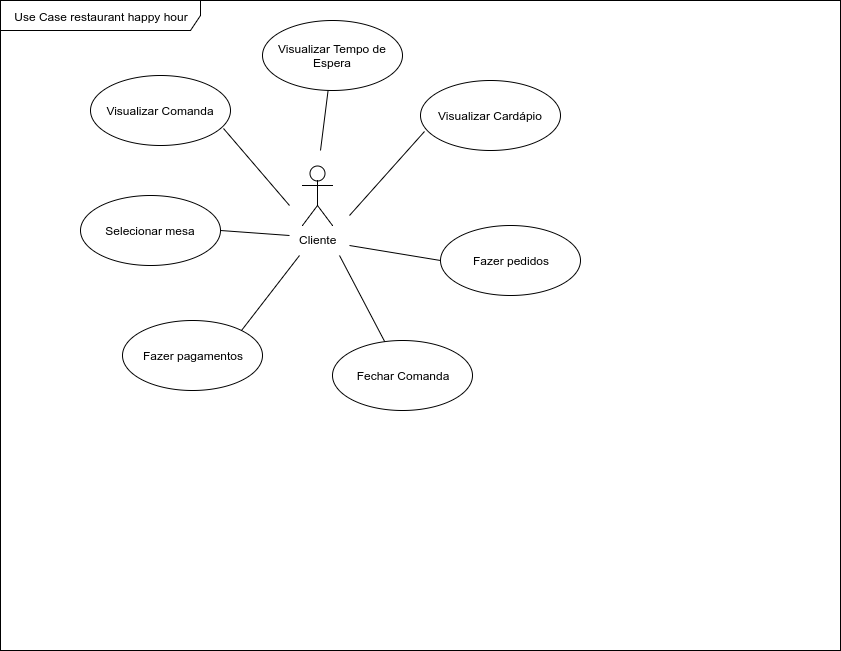
\includegraphics[width=0.6\textwidth]{figuras/diagrama-de-caso-de-uso.png}
	% Caption centralizada
% 	\captionsetup{justification=centering}
	% Caption e fonte 
	 \vspace{-0.2cm}
	\\\textbf{\footnotesize Fonte: Criado pelo autor }
	\label{fig:casodeuso}
\end{figure}
\vspace{-0.5cm}

\subsection{\esp Diagrama de sequência}

A fim de elucidar e facilitar a compreensão do desenvolvimento realçando uma linha temporal das mensagens trocadas entre os objetos do sistema é criado o diagrama de sequência. A partir do diagrama de caso de uso, o diagrama de sequência visa mostrar a sequência de processos realizados pelo usuário entre os diversos objetos do sistema mediante a sua ação ao longo do tempo.

% Figura
\begin{figure}[ht]
	\centering	
	\caption[\hspace{0.1cm}]{Diagrama de sequência}
	\vspace{-0.4cm}
	\includegraphics[width=0.6\textwidth]{figuras/diagrama-de-sequência.png}
	% Caption centralizada
% 	\captionsetup{justification=centering}
	% Caption e fonte 
	 \vspace{-0.2cm}
	\\\textbf{\footnotesize Fonte: Criado pelo autor }
	\label{fig:casodeuso}
\end{figure}
\vspace{-0.5cm}

\subsection{\esp Diagrama de atividade}

A estruturação do fluxo da aplicação e os caminhos possíveis que o usuário pode percorrer dentro do sistema se dá por meio do diagrama de atividade que consiste basicamente de um diagrama de fluxo. Este diagrama possibilita a modelagem de aspectos dinâmicos da aplicação dando um entendimento melhor do funcionando e comportamento do sistema, o que será fundamental para a produção do wireframe.

% Figura
\begin{figure}[ht]
	\centering	
	\caption[\hspace{0.1cm}]{Diagrama de atividade}
	\vspace{-0.4cm}
	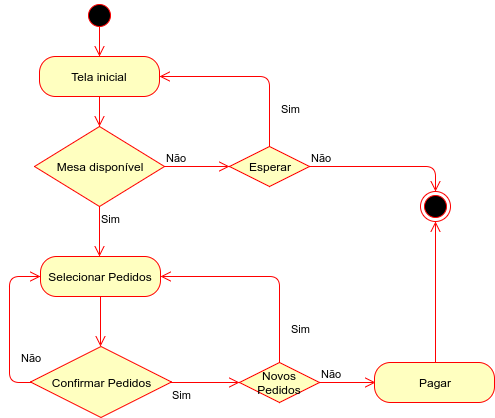
\includegraphics[width=0.6\textwidth]{figuras/diagrama-de-atividade.png}
	% Caption centralizada
% 	\captionsetup{justification=centering}
	% Caption e fonte 
	 \vspace{-0.2cm}
	\\\textbf{\footnotesize Fonte: Criado pelo autor }
	\label{fig:casodeuso}
\end{figure}
\vspace{-0.5cm}

\subsection{\esp Wireframe}

Ao atingir esta etapa do processo de desenvolvimento nos permite criar o wireframe que é um esboço de baixa fidelidade da interface do protótipo. O wireframe permite entender os aspectos visuais, arquitetura da informação e as estruturas da interface, mostrando como será exibido as informações nas telas como menus, botões, estruturas, imagens e formas. É um guia visual para o desenvolvimento das telas.

\subsection{\esp Decisões técnicas e tecnologias}

O desenvolvimento do client-side utilizando a abordagem Progressive Web Apps é obrigatório o uso das tecnologias core da Web: HTML, CSS e Javascript. Devido ao uso da linguagem Javascript o server-side será desenvolvido em Node.js que é interpretador Javascript no lado do servidor. A utilização da linguagem Javascript permite uma implementação isomórfica, ou seja, a mesmo linguagem de programação para toda as etapas de desenvolvimento de ponta a ponta, client-side e server-side.

Portanto, para desenvolver a aplicação é utilizado um conjunto ferramental que utiliza as seguintes tecnologias:

\begin{enumerate}
	\item [1] Visual Studio Code: Editor de texto que será o ambiente de desenvolvimento para implementar a  aplicação com suporte a Javascript, CSS e HTML e outros recursos que auxiliam no desenvolvimento.
	\item [2] Git e github: Ferramentas integradas de versionamento, repositório de arquivos e compartilhamento do código.
	\item [3] Vue.js: Biblioteca que auxilia na criação de SPA, Web Componentes e outros recursos modernos da Web que são utilizados no Progressive Web Apps.
	\item [4] Framework7: Framework para vue.js que disponibiliza componentes UI mobile para ser fidedigna ao wireframe e as tendências de design atual. Os componentes presentes no wireframe que não possuem no framework, será desenvolvido pelo autor.
	\item [5] Node.js: Plataforma desenvolvida em cima do motor Javascript do navegador Google Chrome. Com ele é possível construir facilmente aplicações com rede de forma escalável. Outra característica é o modelo de I/O direcionada a evento não bloqueante que o torna leve e eficiente, sendo ideal para aplicações em tempo real que tem uma massiva troca de dados.
	\item [6] Express:  Framework para node.js que permite de maneira fácil e flexível a criação de aplicações Web robustas e escaláveis utilizando o protocolo HTTP, e aplicando os conceitos de roteamento e middlewares.
	\item [7] MongoDB: Banco de dados não relacional (noSQL) orientado a documentos que utiliza um interface Javascript. A capacidade de armazenar objetos JavaScript nativamente (BSON) economiza tempo e energia de processamento computacional.
	\item [8] Mongoose: ORM MongoDB para node.js.

\end{enumerate}

\subsection{\esp Aplicação server-side}

Web Service é uma solução que procura resolver o problema de comunicação entre aplicações que empregam diferentes tecnologias utilizando protocolos da Internet. A aplicação server-side segue a mesma proposta deste modelo implementando a arquitetura REST no qual utiliza os verbos do protocolo HTTP (GET, POST, DELETE, PUT e PATCH) para definir uma rota que provém recursos e serviços.

O uso do padrão MVC no server-side permite que cada recurso seja gerido de forma independente com características, implementações e responsabilidades distintas no ORM, que por sua vez, retorna os recursos solicitados.  Todo recurso é caracterizado por transações sem estado e são imutáveis para a persistência no banco de dados.

O banco de dados noSQL utiliza o conceito de schema que é uma interface para modelo de documentos. Por ser um conceito relativamente novo na computação, não há uma solução proposta na notação UML da engenharia de software para banco de dados não relacional. Portanto, segundo XXX [32] a modelagem dos dados é baseada em blocos de documentos e subdocumentos, aos quais podem ser referenciados a outros documentos.

% Figura
\begin{figure}[ht]
	\centering	
	\caption[\hspace{0.1cm}]{Diagrama modelagem não relacional MongoDB}
	\vspace{-0.4cm}
	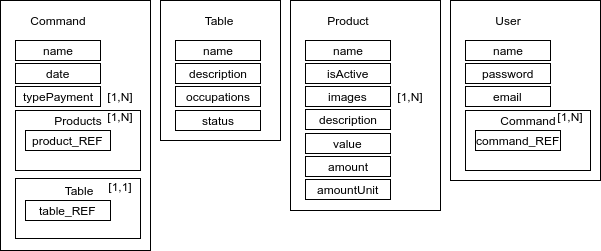
\includegraphics[width=0.6\textwidth]{figuras/diagrama-banco-de-dados.png}
	% Caption centralizada
% 	\captionsetup{justification=centering}
	% Caption e fonte 
	 \vspace{-0.2cm}
	\\\textbf{\footnotesize Fonte: Criado pelo autor }
	\label{fig:casodeuso}
\end{figure}
\vspace{-0.5cm}

\subsection{\esp Aplicação Client-side}

O Vue.js incorpora os princípios da Web moderna usando o padrão MVVM (Model View ViewModel) que é ideal para a implementação da interface do client-side utilizando a abordagem Progressive Web App. A sua separação clara de responsabilidades entre os componentes permite que a aplicação seja modular, flexível, testável e acima de tudo de fácil manutenção.

O uso constante de múltiplos dados, estados, componentes e interações dos recursos torna a manipulação dos dados complexo. O uso de gerenciamento dos dados e estados da aplicação a fim de centralizar e organizar, e paralelamente, fazendo a comunicação com o servidor para que os dados sejam atualizadas permite a consistência de todas as informações. Logo, assim que um dado é alterado na aplicação client-side, é enviado uma requisição para o servidor alterar o mesmo recurso, e consequentemente persistir no banco de dados. Para isso é definido os mesmo schemas (documentos) utilizados no banco de dados, ou seja, o modelo de dados no server-side, é o mesmo modelo no client-side, não necessitando nenhum parseamento, apenas validação dos dados nas camadas de comunicação. Para implementar esse conceito o vue.js utiliza um plugin vuex.

A aplicação é composta por uma única página HTML (index.html), que contém a chamada a todos os ficheiros Javascript e CSS usados, e inicializa a aplicação através do uso da propriedade id="app". Inicializando o componente principal  da aplicação que permite fazer as configurações globais, incorporação dos demais componentes e dependências através do arquivo “main.js” ao qual é codificado de forma a seguir o wireframe proposto.


[IMAGEM]  Print das telas da aplicação para cada tela, explicar o que ela faz

A aplicação utilizando a abordagem Progressive Web Apps se diferencia da abordagem Web Application Mobile pela presença de três tecnologias principais que são elucidadas a seguir:

\begin{enumerate}
	\item [1] localStorage: Permite o armazenamento de dados no dispositivo do cliente. É premissa da abordagem a utilização local dos dados e estados.
	\item [2] Service Works: Permite o funcionamento offline da aplicação. Ela fica como um interceptador da aplicação cliente e servidor. Dentre as propostas dessa API dos browsers modernos é permitir armazenar a aplicação em cache, interceptar pedidos de rede afim de verificar se está online, atualizar a aplicação com a última versão do servidor, mandar notificações (push notifications) e permitir ainda habilitar a execução da aplicação em background.
	\item [3] Web App Manifest: Tem como proposta fornecer características de exibição de aplicação nativa ao navegador para evitar transição muito brusca ao disponibilizar os recursos, e tornar a aplicação instalável. É configurável os ícones da aplicação, nome de identificação e inicialização visual que são mostrados antes do carregamento da aplicação.
\end{enumerate}

\section{\esp RESULTADO E DISCUSSÃO}
Como resultado do trabalho obtivemos resultados relevantes ao utilizar a abordagem Progressive Web Apps no qual foi possível tornar uma página Web em uma aplicação progressiva no qual proporciona o uso dos recursos nativos da plataforma. Utiliza recursos como push notification, tendo navegabilidade fluida, com rápidas interações, usável (mesmo em conexões ruins de rede) e instalável, no qual é criado um ícone na tela inicial do dispositivo do usuário que irá abrir em tela cheia assim como nos aplicativos nativos.

Contudo, a abordagem apresenta desvantagens significativas que devem ser levadas em consideração a sua escolha ao desenvolvimento de uma aplicação mobile. Ao relacionar com as outras abordagens, como já citado  no trabalho, o suporte dos browsers e o desinteresse mercadológico da Apple são pontos relevantes a decisão.

Na tabela abaixo podemos observar a relação entre as abordagens, e em destaque, as evoluções da Web  Mobile para a Progressive Web Apps.


% Tabela
\begin{table}[htb]
	\centering
	\caption{\hspace{0.1cm} Comparative entre as plataformas}
	\vspace{-0.3cm} % espaço entre titulo e tabela
	\label{tab:tabela1}
	% Conteúdo da tabela
	\begin{tabular}{l|c|c}
  \hline
    \textbf{Considerações}	& \textbf{Hibrído} & \textbf{Nativo} & \textbf{Web Mobile} & \textbf{Progressive Web Apps} \\
	\hline
	Esforço para suportar plataformas & Médio & Alto & Baixo & Baixo \\
	Acesso aos recursos do dispositivo & Completo & Completo & Parcial & Parcial (Em expansão) \\	
	Experiência do usuário & Completa & Completa & Média & Completa \\
	Desempenho (Bateria e tempo) & Muito Alto & Muito Alto & Alto & Alto \\
	Atualização do cliente & Necessária & Necessária & Não necessita & Não necessário \\
	Facilidade de publicação & Média & Média & Alta & Alta \\
	Ciclo de aprovação & Em alguns casos & Não existente & Obrigatório & Em alguns casos \\
	Monetização na loja de aplicativos & Disponível & Disponível & Indisponível & Play Store (Em teste) \\	
	Uso Offline & Sim & Sim & Não & Sim \\
	Indexável por mecanismos de busca & Não & Não & Sim & Sim \\
	Notificações locais & Sim & Sim & Não & Sim \\
	Notificações Push & Sim & Sim & Não & Sim \\
	Atualizações rápidas e on-demand & Não & Não & Sim & Sim \\
	Instalável & Sim & Sim & Não & Sim \\
     \hline
 \end{tabular}
 	\vspace{.1cm}  %espaço entre tabela e fonte
	\small
	% Fonte
	{\footnotesize\\ \textbf{Fonte: [12], editado pelo autor}}
\end{table}

Em relação a abordagem Web Mobile, o modelo arquitetural da PWA se dá pela adição e configuração do Service Workers, do arquivo Manifest.json, acesso às APIs nativas pelo browser e o incremento no server-side do PUSH API que envia um Push notification para a aplicação instalada.

% Figura
\begin{figure}[ht]
	\centering	
	\caption[\hspace{0.1cm}]{Modelo arquitetural da Progressive Web App.}
	\vspace{-0.4cm}
	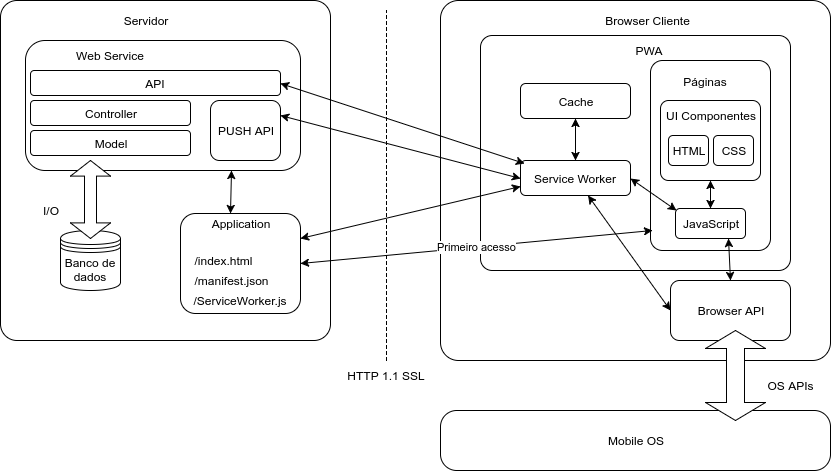
\includegraphics[width=0.6\textwidth]{figuras/arquitetura-pwa.png}
	% Caption centralizada
% 	\captionsetup{justification=centering}
	% Caption e fonte 
	 \vspace{-0.2cm}
	\\\textbf{\footnotesize Fonte: Criado pelo autor }
	\label{fig:casodeuso}
\end{figure}
\vspace{-0.5cm}

Na arquitetura apresentada na figura x, possui dois componentes principais, o servidor e o browser do cliente. A comunicação entre eles se dá pelo Web Service (server-side) através da interface API que trabalha em cima do protocolo de Internet HTTP.

O Web service centraliza e distribui os recursos da aplicação, assim como explicado na seção x.x. A camada Controller é responsável pela regra de negócio da aplicação, que ao término do processamento, passa a responsabilidade para a camada de persistência, Model, gerenciando e persistindo os dados processados no banco de dados. Esse modelo interno desta arquitetura é conhecido como MVC (Model-View-Controller), sendo o View caracterizado pela camada API.

O browser do cliente ao acessar o servidor faz o download dos ativos e renderiza a interface da aplicação graças aos arquivos HTML,  CSS, Javascript ou quaisquer outros recursos estáticos que fornece a estrutura da PWA (client-side). A PWA através do Javascript faz a utilização dos recursos nativos da camada Mobile OS através das APIs do browser.

A camada Service Worker presente na PWA faz o cache e armazenamento da aplicação, que podem ser carregados instantaneamente numa próxima execução. Ao inicializar a aplicação para execução no segundo plano, mesmo a aplicação não estando no primeiro plano, é possível manter contato com o servidor que disponibiliza a camada de PUSH API para o envio de notificações remotas. Toda solicitação HTTP é interceptada pelo Service Worker, ao qual é redirecionada para um recurso em cache, armazenamento local ou para a rede.

A aplicação foi publicada na hospedagem heroku (disponível em http://happy-hour-pwa.heroku.com) e o código fonte e arquivos estão disponíveis no github:

\begin{enumerate}
	\item client-side: https://github.com/henryqrm/happy-hour-client-side
	\item server-side: https://github.com/henryqrm/happy-hour-server-side
\end{enumerate}

\section{\esp CONCLUSÕES E TRABALHOS FUTUROS}

Este trabalho teve como objetivo principal apresentar a abordagem de desenvolvimento Nativo, Híbrida, Web Mobile e a sua evolução, PWA. A partir disso foi desenvolvido um protótipo de solução para casas de Happy Hour utilizando a abordagem PWA e feito as comparações em cima das abordagens apresentadas.

Ao utilizar a linguagem Javascript no client-side e, em seguida, ser capaz de reutilizar a mesma linguagem no servidor em toda a estrutura há uma redução significativa na quantidade de alternância de contexto entre as diversas linguagens de programação que o desenvolvedor precisa compreender, devido a isto, reduz de forma significativa o tempo de desenvolvimento, fato interessante para diminuir custos com equipe e tempo de desenvolvimento.

Diante dos resultados obtidos, e com o desenvolvimento de um protótipo foi possível verificar vantagens e desvantagens ao utilizar a abordagem de desenvolvimento Progressive Web Apps. Por ser relativamente uma abordagem de desenvolvimento recente e com algumas limitações, esta apresenta um enorme potencial em seu uso. Contudo o seu uso hoje deve-se ter cautela, pois ainda há muito o que ser feito para se tornar uma tecnologia sólida e usual no mercado de desenvolvimento mobile. A melhora e evolução contínua das tecnologias core da Web tornará, em um futuro breve, a principal abordagem para o desenvolvimento de aplicações mobile.

Como trabalho futuro decorrente deste poderia ser a comparação do mesmo protótipo em outras abordagens, como a nativa, por exemplo. Ou ainda a evolução do protótipo para uma solução completa, pois é necessário a implementação de funcionalidades e outros requisitos que atendem outros atores que participam do fluxo das casas Happy Hour, como por exemplo o garçom e a cozinha do estabelecimento.
















Os títulos das seções secundárias terão caixa baixa, negrito, tamanho 12.

\subsubsection{\esp Seção terciária}

Caixa baixa, itálico, negrito, tamanho 12.

\subsubsubsection{\esp Seção quartenária}
 
 Caixa baixa, sublinhado, negrito, tamanho 12.
 
 \subsubsubsubsection{\esp Seção quinária}
 
 Nas seções quinárias, deve ser usado caixa baixa, sem negrito, tamanho 12.

\section{\esp Elementos flutuantes}

Elementos inseridos no texto como imagens, tabelas, algoritmos etc.
Recomenda-se a colocação das ilustrações de forma centralizada, dentro das margens. 
Caso não seja possível, em \citeonline{manualpuc} recomenda-se utilizar recursos como: 
 a) utilizar letras com tamanho menor ao padrão do texto; a) imprimir a ilustração no sentido vertical; 
 c) imprimir em folha A3 ou superior e dobrá-la até atingir o tamanho da folha A4. 

Nas normas da PUC é afirmado a necessidade de se observar que todos os elementos flutuantes inseridos devem ter a formatação básica:

\begin{enumerate} 
 \item [a)] Título centralizado localizado na parte superior; 
 \item [a)] Fonte em tamanho 10 na parte inferior;
 \item [c)] Devem ser inseridas o mais próximos do texto que as referenciam.
\end{enumerate}


\subsection{\esp Inserções de ilustrações}

As ilustrações devem ser inseridas seguindo o exemplo da Figura \ref{fig:figura1}. 
% Figura
\begin{figure}[ht]
	\centering	
	\caption[\hspace{0.1cm}Grade Computacional.]{Uma Grade Computacional como fonte transparente}
	\vspace{-0.4cm}
	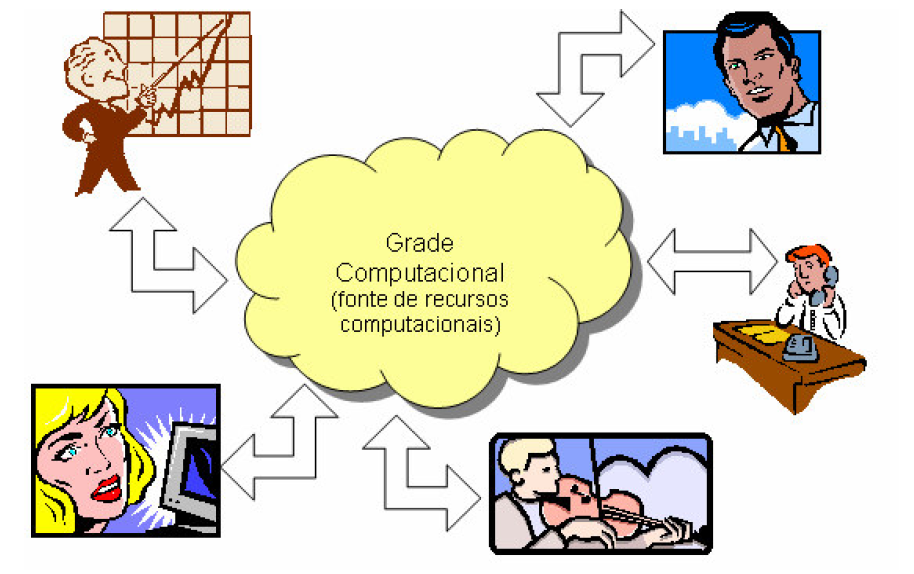
\includegraphics[width=0.6\textwidth]{figuras/grade-comp.png}
	% Caption centralizada
% 	\captionsetup{justification=centering}
	% Caption e fonte 
	 \vspace{-0.2cm}
	\\\textbf{\footnotesize Fonte: \cite{cap-livro} }
	\label{fig:figura1}
\end{figure}
\vspace{-0.5cm}

\subsection{\esp Inserção de tela de software}

Nos casos de telas de \textit{software}, devem ser inseridas como figuras, e referenciadas no texto
como na Figura \ref{fig:tela1}. Além disso, é necessário que seja citada no texto a empresa desenvolvedora.

% Figura
\begin{figure}[!ht]
	\centering	
	\caption[\hspace{0.1cm}Exemplo de tela de software.]{Exemplo de tela de software}
	  \vspace{-0.4cm}
	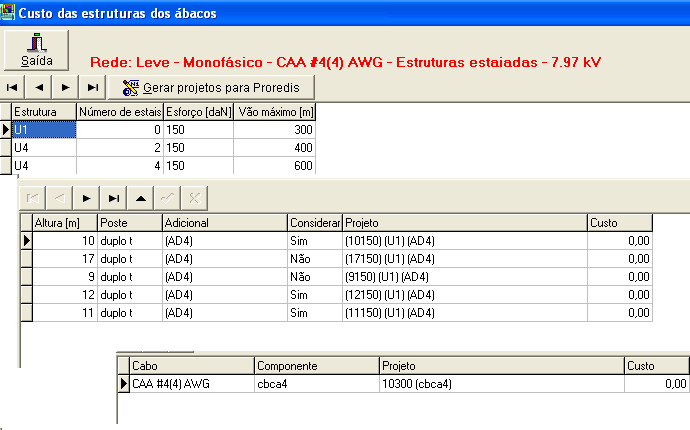
\includegraphics[width=.8\textwidth]{figuras/tela1.png}
	% Caption centralizada
% 	\captionsetup{justification=centering}
	% Caption e fonte
	 \vspace{-0.3cm}
	\\\textbf{\footnotesize Fonte: \cite{tela1}}
	\label{fig:tela1}
\end{figure}

\subsection{\esp Inserção de gráficos e mapas}

O gráfico é um tipo de ilustração que deve conter todos os elementos citados e também a descrição de seu título
diferenciando-o das figuras da mesma forma que no Gráfico 1. 

\begin{center}
	\centering	
 	\textbf{Gráfico 1 - Exemplo de um gráfico} \\
%  	  \vspace{0.cm}
	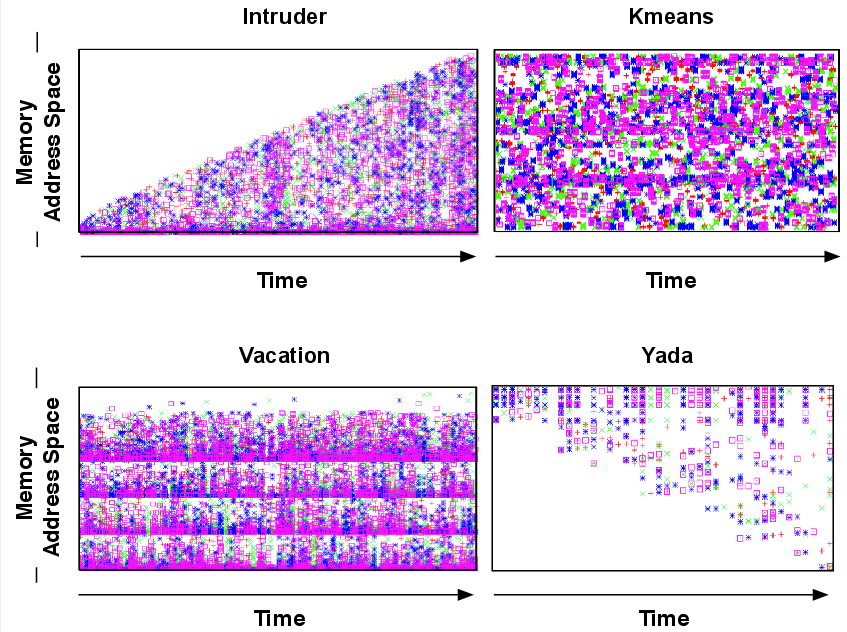
\includegraphics[width=0.7\textwidth]{figuras/access.png}
	% Caption centralizada
% 	\captionsetup{justification=centering}
	% Caption e fonte
	 \vspace{-0.3cm}
	\\\textbf{\footnotesize Fonte: \cite{tese}}
	\label{grafico1}
\end{center}

A mesma regra se aplica para mapas, que devem ser adicionados seguindo as regras de apresentação já mostradas. No caso específico,
o título e a numeração, também como os gráficos, devem começar do numeral ``1'' depois da marcação ``Mapa'' seguido do nome do elemento.
Exemplo: \textbf{Mapa 1 - Exemplo de um Mapa}.

 \subsection{\esp Tabelas}

As tabelas são fechadas nas laterais. Entre os elementos da tabela devem haver linhas. Um exemplo é a Tabela \ref{tab:tabela1}. 

% Tabela
\begin{table}[htb]
	\centering
	\caption{\hspace{0.1cm} Exemplo de uma tabela}
	\vspace{-0.3cm} % espaço entre titulo e tabela
	\label{tab:tabela1}
	% Conteúdo da tabela
	\begin{tabular}{l|c|c}
  \hline
    \textbf{Imagem}	& \textbf{transferência} & \textbf{tempo} \\
    \hline
     estação 1	& 7,72 MB/s &  1:22:18 \\
     estação 2	& 7,72 MB/s &  1:22:17 \\
     estação 3	& 7,59 MB/s & 1:24:25 \\
     estação 4  & 7,53 MB/s & 1:43:27 \\
     estação 5	& 6,14 MB/s  &  1:24:41 \\
     estação 6  &  7,50 MB/s & 1:23:53 \\
     estação 7  & 7,58 MB/s  &  1:24:02 \\
     estação 8  & 7,8 MB/s  &  1:29:06 \\
     estação 9  & 7,9 MB/s  &  1:30:05 \\
     estação 10 & 8,0 MB/s  &  1:32:03 \\
     \hline
 \end{tabular}
 	\vspace{.1cm}  %espaço entre tabela e fonte
	\small
	% Fonte
	{\footnotesize\\ \textbf{Fonte: \cite{monog-fabio}}}
\end{table}

\subsection{\esp Quadros}

Os quadros diferem das tabelas por apresentarem dados textuais.
Esses dados podem ser esquemáticos, comparativos ou descritivos.

   \begin{center}
          \centering
       	\textbf{Quadro 1 - Bandas/Artistas de Rock e outros}\\
% 	\vspace{-0.3cm} % espaço entre titulo e tabela
        \label{quadro1}
	\begin{tabular}{|c|c|c|c|} \hline
	\multicolumn{4}{|c|}{\textbf{Bandas ou Artigas de Rock e outros}} 	  \\ 
		\hline \textbf{	Progressivo} & Pink Floyd & Jethro Tull	& Yesterday \\ 
		 \hline \textbf{ Metal}  & Metallica & Iron Maidam & Black Sabath \\ 
		\hline \textbf{	Arena Rock} & Led Zeppelin & The Rolling Stones & Beatles \\ 
		\hline \textbf{ Punk} & Ramones & Black Flag & NOFX	\\ 
		\hline \textbf{	Nacional} & Ira & Engenheiros & Vinil	\\ 
		\hline \textbf{	S.J.E.} & Apolo XI & Invasão 7 & Por do Sol \\ 
		\hline \textbf{	Grunge} & Nirvana & Pear Jam & Alice in Chains	\\ 
		\hline \textbf{	Rock Folk} & Bod Dylan & The Byrds &  The Mamas \& the Papas \\
		\hline \textbf{	Blues} & B.B. King & Albert Colins & Mady Wathers \\ 
		\hline \textbf{	New Wave} & The Police & The Pretenders, &  Duran Duran\\ 
 		\hline \textbf{	Rock Folk} & Bod Dylan & The Byrds &  The Mamas \& the Papas \\
 		\hline \textbf{	Rock alternativo} & R.E.M.& Hüsker Dü & Big Black\\ 
 		
		\hline
	\end{tabular}
	\vspace{0.1cm} 
	{\footnotesize\\ \textbf{Fonte: Dados da pesquisa}}
   \end{center}

Para gráficos, quadros e tabelas, cujos dados foram extraídos da própria pesquisa, 
 usar a expressão: Dados da pesquisa. Ver exemplo no Quadro 1.
   

\subsection{\esp Inserção de algoritmos}

Para inserir um algoritmo, utilizar o exemplo do Algoritmo  \ref{alg:rnagenerica}.
Todos os algoritmos devem ser inseridos como figura, indicada por nome e  fonte. Caso 
forem de própria autoria, isso deverá ser mencionado na fonte, como elaboração feita pelos autores.

% algoritmo
% \begin{figure}[ht]
\begin{center}	
	% Arquivo da figura
% 	\caption[\hspace{0.1cm} Texto da figuras.]{Algorítmo CAC RD Neural}
         \textbf{Algoritmo 1 -  CAC RD Neural}
	\vspace{-0.3cm}
\begin{minipage}[ht]{13cm}
\begin{algorithm}[H]
  \footnotesize
  \caption{CAC-RD Neural}
  \label{alg:rnagenerica}
  \begin{algorithmic}[1]
      \STATE \textbf{Entrada:} Requisição da chamada
    \STATE \textbf{Saída:} Aceitação ou bloqueio da solicitação
    
    \STATE Preenche o vetor de $attributes.size+1$ atributos com os valores dos atributos, sendo a primeira posição do vetor preenchida com o valor 1
		\STATE $hidden\_layer\_size =  attributes.size*2+1;$

    \FOR{$i$ = 1 to $attributes.size+1$}
    	\STATE \textbf{normalizar}($Entrada_i$)
    \ENDFOR

		\STATE $double [] net = new double [hidden\_layer\_size];$
    \STATE $net = hidden\_layer\_weights * attributes;$
   	\FOR{$i$ = 0 to hidden\_layer\_size}
			\STATE $net [i] = 1.0 / (1.0 + exp((-1.0)*net[i]));$
		\ENDFOR

		\STATE $double [] ipVector = new double [hidden\_layer\_size+1];$
    \STATE $ipVector [0] = 1.0;$
   	\FOR{$i$ = 1 to $hidden\_layer\_size+1$}
			\STATE $ipVector [i] = net [i-1];$
		\ENDFOR
		
		\STATE $output = output\_layer\_weights *  ipVector;$
    \STATE output = \textbf{desnormalizar}(Saída)
    \STATE \textbf{net\_update} (requisition);
    
    \STATE \textbf{Retorna} output; FIM
  \end{algorithmic}
\end{algorithm}
% \vspace{-0.3cm} % espaço entre algoritmo e fonte

\small \centering \textbf{\footnotesize Fonte: \cite{mestrado}.}
\end{minipage}
\end{center}
% \end{figure}

Para ilustrações criadas ou adaptadas a partir de outras ilustrações, usar as expressões: 
“Adaptado de...” ou “Criado pelo autor`` com dados extraídos de \ldots
   
   
\section{\esp CITAÇÕES}


Referências deverão ser adicionadas no arquivo \textit{bibliografia.bib}. Cada referência deverá ser adicionada conforme o padrão de normalização da PUC, 
o qual poderá ser consultado na página da biblioteca da PUC Minas \cite{manualpuc}. Todas as publicações citadas no texto deverão ter correspondente nas referências, 
e as indicações de autoria da citação e do ano deverão ser idênticas aos dados expostos.


\subsection{\esp Citação livre ou indireta}

Quando se reproduzir ideias, sem transcrever as palavras do autor, a indicação da página é opcional. Exemplos desse tipo de citação:
\begin{enumerate} 
 \item [a)] Citação com um autor \cite{knuth}. 
 \item [b)] Citação de artigos em revistas com dois autores \cite{artigo01}.
  \item [c)] Trabalho em congresso com três autores \cite{dovzan:01}.
 \item [d)] Trabalhos com mais de três autores \cite{cap-livro}.
 \item [e)] Dois autores em duas obras distintas \cite{knuth,groupp}.
 \item [d)] Trabalhos distintos com vários autores \cite{congresso,cap-livro}.
 
\end{enumerate}

\subsection{\esp Citação direta ou textual}

Transcrição literal de textos de outros autores. Nesse caso, deverão ser especificadas as páginas consultadas. 
Se desejar, poderão ser grafadas em itálico para melhor visualização.

\subsubsection{\esp Textual Curtas}

Quando curtas (até 3 linhas) serão inseridas na sequência normal do texto, entre aspas com as mesma formatação.

\subsubsection{\esp Textual Longas}

Citações longas (mais de 3 linhas) deverão constituir um parágrafo independente, recuado a 4 cm da margem esquerda, 
com letra tamanho 10 e digitado em espaço simples, sem aspas.
\begin{citacaodireta}
Hegel chama trabalho à forma específica da satisfação das necessidades, que
distingue da natureza o espírito existente. Assim como a linguagem infringe
a imposição da intuição e ordena o caos das múltiplas sensações em coisas
identificáveis, assim o trabalho infringe a imposição do \hspace{0.1cm}desejo \hspace{0.1cm}imediato \hspace{0.1cm}e
suspende, por assim dizer, o processo de satisfação das necessidades.
\cite[25]{habermas}.
\end{citacaodireta}


% Artigo \cite{whatershed:01}

\subsubsection{\esp Textual de outros idiomas (Tradução)}

\begin{citacaodireta} 
Um \textit{cluster} é um computador paralelo construído de componentes e processos de \textit{software} (tal como sistema de \textit{software}). 
Um \textit{cluster} é formado de nós, cada um contendo um ou mais processadores, memória que é compartilhada por todos os processadores do nodo 
(somente eles), e dispositivos periféricos adicionais (tais como discos), conectados pela rede e que permitem tráfego de dados entre os nós...
\cite[p. 10, tradução nossa]{groupp}\footnote {  … a cluster is a parallel computer that is constructed of commodity  componets and runs 
(as its system software) commodity software. A cluster is made of nodes, each conteining one or more processors, memory that is  shared 
by all of the processors in (and only on) the node, and addtional peripheral devices (surch as disks),
 connected by network that allows data to move between the nodes}.
\end{citacaodireta}
 
\subsection{\esp Exemplos de citações} 

Alguns exemplos de citações mais utilizadas e/ou que geram algumas dúvidas. É válido observar que não citaremos
todas as possibilidades de citações da norma da PUC Minas, sendo assim é de extrema relevância que se consulte 
o documento no site da Biblioteca da PUC Minas para maiores esclarecimentos acerca de citações \cite{manualpuc}.

\subsubsection{\esp Citação de monografia, dissertação e tese}

Exemplo de citação de monografia de curso de graduação ou especialização pode ser vista em \citeonline{monog-fabio}.
Exemplo de dissertação de mestrado é referida como \citeonline{mestrado}.

Para o caso de doutorado é citado da seguinte forma, Góes (\citeyear{tese}). Nesse exemplo é válido observar a forma
como está escrito no documento \LaTeX, pois citações que compreendem no texto o nome do autor como sua parte, necessitam 
do parâmetro \verb$\citeonline{}$. 

\subsubsection{\esp Livros e partes de livros}

Exemplo de capítulo de livro fica conforme este exemplo \cite{cap-livro}.

Para livros citados no corpo do texto e com duas citações juntas, ver os exemplos \citeonline{knuth,groupp}.
Caso essa citação não fizesse parte do texto será referencia dessa forma \cite{knuth,groupp}.

Citações institucionais ou documentos técnicos de alguma entidade devem ser citados desta forma \cite{pmbok}.

\subsubsection{\esp Tela de software}

Para  citar a tela de um \textit{software} faça da seguinte forma, \citeonline{tela1}.

\subsubsection{\esp Citações da Biblia Sagrada}

A Bíblia está dividida em duas grandes partes: O Antigo Testamento e o Novo Testamento, divididos em livros, capítulos e versículos. 
Portanto, a citação de partes da Bíblia deve apresentar o título do livro de forma abreviada ou por extenso, o número do capítulo e o número do versículo.


\begin{citacaodireta}
Moisés estendeu a mão sobre o mar. Com um forte \hspace{-0.1cm} vento \hspace{0.1cm} leste a \hspace{0.1cm}sobrar a
noite toda, o Senhor repeliu o mar e o pôs a seco. As águas se fenderam e
os filhos de Israel entraram no meio do mar a pé enxuto, enquanto as águas
formavam uma muralha à direita e à esquerda deles (\citeauthor{biblia} 14,21).
\end{citacaodireta}

\subsection{\esp Conclusão}

Discussão dos resultados obtidos na pesquisa. É onde se colocam as observações do autor. 
Poderá também apresentar sugestões de novas linhas de estudo.

A conclusão deve estar de acordo com os objetivos do trabalho.

A conclusão não deve apresentar citações ou interpretações de outros autores.

% \subsection{\esp Trabalhos futuros}
% 
% Sugestões de estudos posteriores são ser adicionados subseção deste capítulo de conclusão.
